\begin{figure}[!t]
\centering
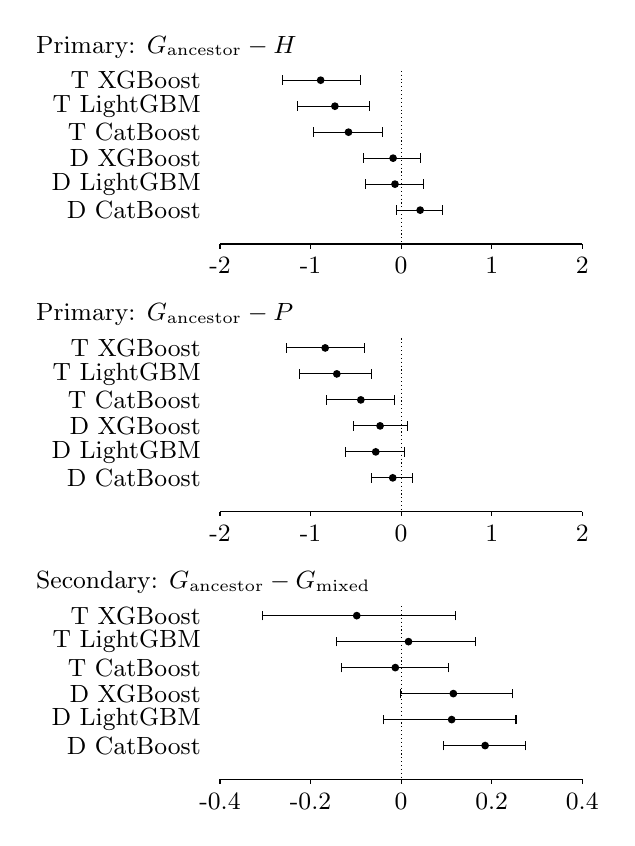
\begin{tikzpicture}[x=1cm,y=1cm]
\small
\node[anchor=west] at (0,-0.000) {Primary: $G_{\mathrm{ancestor}}-H$};
\node[anchor=east] at (2.32,-0.420) {T XGBoost};
\draw (3.2385,-0.420) -- (4.2323,-0.420);
\draw (3.2385,-0.480) -- (3.2385,-0.360);
\draw (4.2323,-0.480) -- (4.2323,-0.360);
\fill (3.7279,-0.420) circle (1.4pt);
\node[anchor=east] at (2.32,-0.750) {T LightGBM};
\draw (3.4320,-0.750) -- (4.3469,-0.750);
\draw (3.4320,-0.810) -- (3.4320,-0.690);
\draw (4.3469,-0.810) -- (4.3469,-0.690);
\fill (3.9088,-0.750) circle (1.4pt);
\node[anchor=east] at (2.32,-1.080) {T CatBoost};
\draw (3.6377,-1.080) -- (4.5131,-1.080);
\draw (3.6377,-1.140) -- (3.6377,-1.020);
\draw (4.5131,-1.140) -- (4.5131,-1.020);
\fill (4.0813,-1.080) circle (1.4pt);
\node[anchor=east] at (2.32,-1.410) {D XGBoost};
\draw (4.2665,-1.410) -- (4.9967,-1.410);
\draw (4.2665,-1.470) -- (4.2665,-1.350);
\draw (4.9967,-1.470) -- (4.9967,-1.350);
\fill (4.6478,-1.410) circle (1.4pt);
\node[anchor=east] at (2.32,-1.740) {D LightGBM};
\draw (4.2961,-1.740) -- (5.0390,-1.740);
\draw (4.2961,-1.800) -- (4.2961,-1.680);
\draw (5.0390,-1.800) -- (5.0390,-1.680);
\fill (4.6719,-1.740) circle (1.4pt);
\node[anchor=east] at (2.32,-2.070) {D CatBoost};
\draw (4.6866,-2.070) -- (5.2736,-2.070);
\draw (4.6866,-2.130) -- (4.6866,-2.010);
\draw (5.2736,-2.130) -- (5.2736,-2.010);
\fill (4.9917,-2.070) circle (1.4pt);
\draw[densely dotted] (4.7500,-0.300) -- (4.7500,-2.500);
\draw (2.45,-2.500) -- (7.05,-2.500);
\draw (2.4500,-2.500) -- (2.4500,-2.560) node[below] {-2};
\draw (3.6000,-2.500) -- (3.6000,-2.560) node[below] {-1};
\draw (4.7500,-2.500) -- (4.7500,-2.560) node[below] {0};
\draw (5.9000,-2.500) -- (5.9000,-2.560) node[below] {1};
\draw (7.0500,-2.500) -- (7.0500,-2.560) node[below] {2};
\node[anchor=west] at (0,-3.400) {Primary: $G_{\mathrm{ancestor}}-P$};
\node[anchor=east] at (2.32,-3.820) {T XGBoost};
\draw (3.2982,-3.820) -- (4.2878,-3.820);
\draw (3.2982,-3.880) -- (3.2982,-3.760);
\draw (4.2878,-3.880) -- (4.2878,-3.760);
\fill (3.7857,-3.820) circle (1.4pt);
\node[anchor=east] at (2.32,-4.150) {T LightGBM};
\draw (3.4620,-4.150) -- (4.3758,-4.150);
\draw (3.4620,-4.210) -- (3.4620,-4.090);
\draw (4.3758,-4.210) -- (4.3758,-4.090);
\fill (3.9330,-4.150) circle (1.4pt);
\node[anchor=east] at (2.32,-4.480) {T CatBoost};
\draw (3.7965,-4.480) -- (4.6691,-4.480);
\draw (3.7965,-4.540) -- (3.7965,-4.420);
\draw (4.6691,-4.540) -- (4.6691,-4.420);
\fill (4.2381,-4.480) circle (1.4pt);
\node[anchor=east] at (2.32,-4.810) {D XGBoost};
\draw (4.1407,-4.810) -- (4.8299,-4.810);
\draw (4.1407,-4.870) -- (4.1407,-4.750);
\draw (4.8299,-4.870) -- (4.8299,-4.750);
\fill (4.4825,-4.810) circle (1.4pt);
\node[anchor=east] at (2.32,-5.140) {D LightGBM};
\draw (4.0443,-5.140) -- (4.7953,-5.140);
\draw (4.0443,-5.200) -- (4.0443,-5.080);
\draw (4.7953,-5.200) -- (4.7953,-5.080);
\fill (4.4275,-5.140) circle (1.4pt);
\node[anchor=east] at (2.32,-5.470) {D CatBoost};
\draw (4.3784,-5.470) -- (4.8995,-5.470);
\draw (4.3784,-5.530) -- (4.3784,-5.410);
\draw (4.8995,-5.530) -- (4.8995,-5.410);
\fill (4.6434,-5.470) circle (1.4pt);
\draw[densely dotted] (4.7500,-3.700) -- (4.7500,-5.900);
\draw (2.45,-5.900) -- (7.05,-5.900);
\draw (2.4500,-5.900) -- (2.4500,-5.960) node[below] {-2};
\draw (3.6000,-5.900) -- (3.6000,-5.960) node[below] {-1};
\draw (4.7500,-5.900) -- (4.7500,-5.960) node[below] {0};
\draw (5.9000,-5.900) -- (5.9000,-5.960) node[below] {1};
\draw (7.0500,-5.900) -- (7.0500,-5.960) node[below] {2};
\node[anchor=west] at (0,-6.800) {Secondary: $G_{\mathrm{ancestor}}-G_{\mathrm{mixed}}$};
\node[anchor=east] at (2.32,-7.220) {T XGBoost};
\draw (2.9845,-7.220) -- (5.4389,-7.220);
\draw (2.9845,-7.280) -- (2.9845,-7.160);
\draw (5.4389,-7.280) -- (5.4389,-7.160);
\fill (4.1863,-7.220) circle (1.4pt);
\node[anchor=east] at (2.32,-7.550) {T LightGBM};
\draw (3.9301,-7.550) -- (5.6971,-7.550);
\draw (3.9301,-7.610) -- (3.9301,-7.490);
\draw (5.6971,-7.610) -- (5.6971,-7.490);
\fill (4.8436,-7.550) circle (1.4pt);
\node[anchor=east] at (2.32,-7.880) {T CatBoost};
\draw (3.9932,-7.880) -- (5.3536,-7.880);
\draw (3.9932,-7.940) -- (3.9932,-7.820);
\draw (5.3536,-7.940) -- (5.3536,-7.820);
\fill (4.6762,-7.880) circle (1.4pt);
\node[anchor=east] at (2.32,-8.210) {D XGBoost};
\draw (4.7390,-8.210) -- (6.1605,-8.210);
\draw (4.7390,-8.270) -- (4.7390,-8.150);
\draw (6.1605,-8.270) -- (6.1605,-8.150);
\fill (5.4131,-8.210) circle (1.4pt);
\node[anchor=east] at (2.32,-8.540) {D LightGBM};
\draw (4.5229,-8.540) -- (6.2089,-8.540);
\draw (4.5229,-8.600) -- (4.5229,-8.480);
\draw (6.2089,-8.600) -- (6.2089,-8.480);
\fill (5.3916,-8.540) circle (1.4pt);
\node[anchor=east] at (2.32,-8.870) {D CatBoost};
\draw (5.2924,-8.870) -- (6.3288,-8.870);
\draw (5.2924,-8.930) -- (5.2924,-8.810);
\draw (6.3288,-8.930) -- (6.3288,-8.810);
\fill (5.8166,-8.870) circle (1.4pt);
\draw[densely dotted] (4.7500,-7.100) -- (4.7500,-9.300);
\draw (2.45,-9.300) -- (7.05,-9.300);
\draw (2.4500,-9.300) -- (2.4500,-9.360) node[below] {-0.4};
\draw (3.6000,-9.300) -- (3.6000,-9.360) node[below] {-0.2};
\draw (4.7500,-9.300) -- (4.7500,-9.360) node[below] {0};
\draw (5.9000,-9.300) -- (5.9000,-9.360) node[below] {0.2};
\draw (7.0500,-9.300) -- (7.0500,-9.360) node[below] {0.4};
\end{tikzpicture}
\caption{All prespecified AP differences, in percentage points (100 times the fraction difference). T and D denote turf and dirt. Points average paired seed-specific differences; whiskers are descriptive 95\% paired whole-race bootstrap percentile intervals, conditional on the fitted models and unadjusted for multiple comparisons. Panels use their indicated scales. The test was previously examined. Denominators and coverage are in Tables~\ref{tab:cohort} and \ref{tab:focused_coverage}.}
\label{fig:focused_contrasts}
\end{figure}
